\documentclass{standalone}
\usepackage{tikz}
% create a new adjust box
\usepackage{tikzscale}
\usepackage{lscape}
\usepackage{tikz}
% use to adjust the positionS
\usetikzlibrary{positioning}
\usetikzlibrary{calc}
\tikzset{abs1/.style={xshift=3cm,yshift=2cm}}
\usetikzlibrary{shapes.geometric,arrows}
\tikzstyle{arrow}=
[thick,->,>=stealth]


\begin{document}
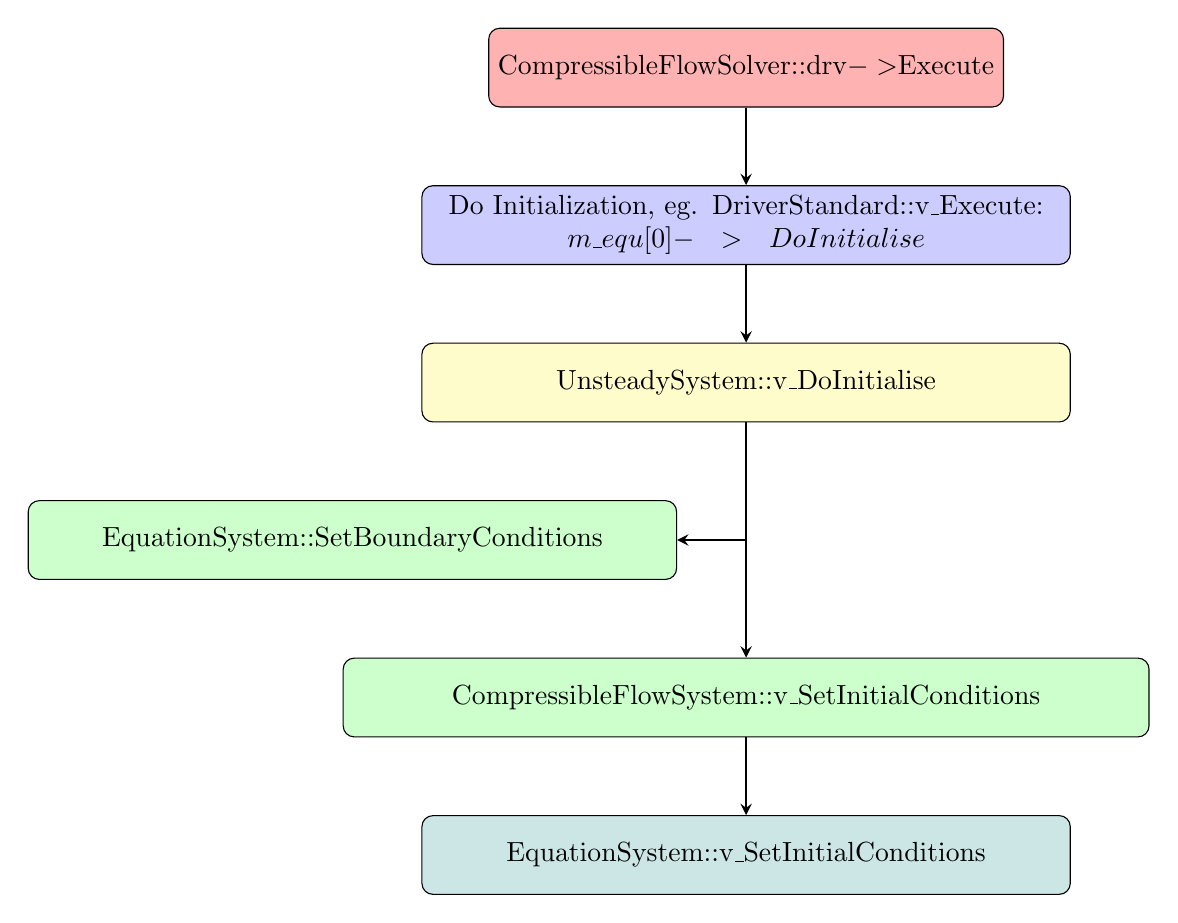
\begin{tikzpicture}[scale=0.2,node distance=2cm]
\node (A)
[rectangle,
rounded corners,
minimum width=3cm,
minimum height=1cm,
text centered,
draw=black,
fill=red!30]
{CompressibleFlowSolver::drv$->$Execute};
\node (B)
[rectangle,
rounded corners,
minimum width=8cm,
minimum height=1cm,
text width=8cm,
text centered,
draw=black,
fill=blue!20,
below of=A,
xshift=0cm,
yshift=0cm]
{Do Initialization, eg. DriverStandard::v$\_$Execute: $m\_equ[0]->DoInitialise$};
\draw[arrow](A)--(B);
\node (C)
[rectangle,
rounded corners,
minimum width=8cm,
minimum height=1cm,
text width=8cm,
text centered,
draw=black,
fill=yellow!20,
below of=B,
xshift=0cm,
yshift=0cm]
{UnsteadySystem::v$\_$DoInitialise};
\draw[arrow](B)--(C);
\node (D_1)
[rectangle,
rounded corners,
minimum width=8cm,
minimum height=1cm,
text width=8cm,
text centered,
draw=black,
fill=green!20,
below of=C,
xshift=-5cm,
yshift=0cm]
{EquationSystem::SetBoundaryConditions};
\draw[arrow](C)|-(D_1);
\node (D_2)
[rectangle,
rounded corners,
minimum width=10cm,
minimum height=1cm,
text width=10cm,
text centered,
draw=black,
fill=green!20,
below of=C,
xshift=0cm,
yshift=-2cm]
{CompressibleFlowSystem::v$\_$SetInitialConditions};
\draw[arrow](C)--(D_2);
\node (E_1)
[rectangle,
rounded corners,
minimum width=8cm,
minimum height=1cm,
text width=8cm,
text centered,
draw=black,
fill=teal!20,
below of=D_2,
xshift=0cm,
yshift=0cm]
{EquationSystem::v$\_$SetInitialConditions};
\draw[arrow](D_2)--(E_1);
\end{tikzpicture}
\end{document}